% Options for packages loaded elsewhere
\PassOptionsToPackage{unicode}{hyperref}
\PassOptionsToPackage{hyphens}{url}
\PassOptionsToPackage{dvipsnames,svgnames,x11names}{xcolor}
%
\documentclass[
  letterpaper,
  DIV=11,
  numbers=noendperiod]{scrreprt}

\usepackage{amsmath,amssymb}
\usepackage{lmodern}
\usepackage{iftex}
\ifPDFTeX
  \usepackage[T1]{fontenc}
  \usepackage[utf8]{inputenc}
  \usepackage{textcomp} % provide euro and other symbols
\else % if luatex or xetex
  \usepackage{unicode-math}
  \defaultfontfeatures{Scale=MatchLowercase}
  \defaultfontfeatures[\rmfamily]{Ligatures=TeX,Scale=1}
\fi
% Use upquote if available, for straight quotes in verbatim environments
\IfFileExists{upquote.sty}{\usepackage{upquote}}{}
\IfFileExists{microtype.sty}{% use microtype if available
  \usepackage[]{microtype}
  \UseMicrotypeSet[protrusion]{basicmath} % disable protrusion for tt fonts
}{}
\makeatletter
\@ifundefined{KOMAClassName}{% if non-KOMA class
  \IfFileExists{parskip.sty}{%
    \usepackage{parskip}
  }{% else
    \setlength{\parindent}{0pt}
    \setlength{\parskip}{6pt plus 2pt minus 1pt}}
}{% if KOMA class
  \KOMAoptions{parskip=half}}
\makeatother
\usepackage{xcolor}
\setlength{\emergencystretch}{3em} % prevent overfull lines
\setcounter{secnumdepth}{5}
% Make \paragraph and \subparagraph free-standing
\ifx\paragraph\undefined\else
  \let\oldparagraph\paragraph
  \renewcommand{\paragraph}[1]{\oldparagraph{#1}\mbox{}}
\fi
\ifx\subparagraph\undefined\else
  \let\oldsubparagraph\subparagraph
  \renewcommand{\subparagraph}[1]{\oldsubparagraph{#1}\mbox{}}
\fi

\usepackage{color}
\usepackage{fancyvrb}
\newcommand{\VerbBar}{|}
\newcommand{\VERB}{\Verb[commandchars=\\\{\}]}
\DefineVerbatimEnvironment{Highlighting}{Verbatim}{commandchars=\\\{\}}
% Add ',fontsize=\small' for more characters per line
\usepackage{framed}
\definecolor{shadecolor}{RGB}{241,243,245}
\newenvironment{Shaded}{\begin{snugshade}}{\end{snugshade}}
\newcommand{\AlertTok}[1]{\textcolor[rgb]{0.68,0.00,0.00}{#1}}
\newcommand{\AnnotationTok}[1]{\textcolor[rgb]{0.37,0.37,0.37}{#1}}
\newcommand{\AttributeTok}[1]{\textcolor[rgb]{0.40,0.45,0.13}{#1}}
\newcommand{\BaseNTok}[1]{\textcolor[rgb]{0.68,0.00,0.00}{#1}}
\newcommand{\BuiltInTok}[1]{\textcolor[rgb]{0.00,0.23,0.31}{#1}}
\newcommand{\CharTok}[1]{\textcolor[rgb]{0.13,0.47,0.30}{#1}}
\newcommand{\CommentTok}[1]{\textcolor[rgb]{0.37,0.37,0.37}{#1}}
\newcommand{\CommentVarTok}[1]{\textcolor[rgb]{0.37,0.37,0.37}{\textit{#1}}}
\newcommand{\ConstantTok}[1]{\textcolor[rgb]{0.56,0.35,0.01}{#1}}
\newcommand{\ControlFlowTok}[1]{\textcolor[rgb]{0.00,0.23,0.31}{#1}}
\newcommand{\DataTypeTok}[1]{\textcolor[rgb]{0.68,0.00,0.00}{#1}}
\newcommand{\DecValTok}[1]{\textcolor[rgb]{0.68,0.00,0.00}{#1}}
\newcommand{\DocumentationTok}[1]{\textcolor[rgb]{0.37,0.37,0.37}{\textit{#1}}}
\newcommand{\ErrorTok}[1]{\textcolor[rgb]{0.68,0.00,0.00}{#1}}
\newcommand{\ExtensionTok}[1]{\textcolor[rgb]{0.00,0.23,0.31}{#1}}
\newcommand{\FloatTok}[1]{\textcolor[rgb]{0.68,0.00,0.00}{#1}}
\newcommand{\FunctionTok}[1]{\textcolor[rgb]{0.28,0.35,0.67}{#1}}
\newcommand{\ImportTok}[1]{\textcolor[rgb]{0.00,0.46,0.62}{#1}}
\newcommand{\InformationTok}[1]{\textcolor[rgb]{0.37,0.37,0.37}{#1}}
\newcommand{\KeywordTok}[1]{\textcolor[rgb]{0.00,0.23,0.31}{#1}}
\newcommand{\NormalTok}[1]{\textcolor[rgb]{0.00,0.23,0.31}{#1}}
\newcommand{\OperatorTok}[1]{\textcolor[rgb]{0.37,0.37,0.37}{#1}}
\newcommand{\OtherTok}[1]{\textcolor[rgb]{0.00,0.23,0.31}{#1}}
\newcommand{\PreprocessorTok}[1]{\textcolor[rgb]{0.68,0.00,0.00}{#1}}
\newcommand{\RegionMarkerTok}[1]{\textcolor[rgb]{0.00,0.23,0.31}{#1}}
\newcommand{\SpecialCharTok}[1]{\textcolor[rgb]{0.37,0.37,0.37}{#1}}
\newcommand{\SpecialStringTok}[1]{\textcolor[rgb]{0.13,0.47,0.30}{#1}}
\newcommand{\StringTok}[1]{\textcolor[rgb]{0.13,0.47,0.30}{#1}}
\newcommand{\VariableTok}[1]{\textcolor[rgb]{0.07,0.07,0.07}{#1}}
\newcommand{\VerbatimStringTok}[1]{\textcolor[rgb]{0.13,0.47,0.30}{#1}}
\newcommand{\WarningTok}[1]{\textcolor[rgb]{0.37,0.37,0.37}{\textit{#1}}}

\providecommand{\tightlist}{%
  \setlength{\itemsep}{0pt}\setlength{\parskip}{0pt}}\usepackage{longtable,booktabs,array}
\usepackage{calc} % for calculating minipage widths
% Correct order of tables after \paragraph or \subparagraph
\usepackage{etoolbox}
\makeatletter
\patchcmd\longtable{\par}{\if@noskipsec\mbox{}\fi\par}{}{}
\makeatother
% Allow footnotes in longtable head/foot
\IfFileExists{footnotehyper.sty}{\usepackage{footnotehyper}}{\usepackage{footnote}}
\makesavenoteenv{longtable}
\usepackage{graphicx}
\makeatletter
\def\maxwidth{\ifdim\Gin@nat@width>\linewidth\linewidth\else\Gin@nat@width\fi}
\def\maxheight{\ifdim\Gin@nat@height>\textheight\textheight\else\Gin@nat@height\fi}
\makeatother
% Scale images if necessary, so that they will not overflow the page
% margins by default, and it is still possible to overwrite the defaults
% using explicit options in \includegraphics[width, height, ...]{}
\setkeys{Gin}{width=\maxwidth,height=\maxheight,keepaspectratio}
% Set default figure placement to htbp
\makeatletter
\def\fps@figure{htbp}
\makeatother
\newlength{\cslhangindent}
\setlength{\cslhangindent}{1.5em}
\newlength{\csllabelwidth}
\setlength{\csllabelwidth}{3em}
\newlength{\cslentryspacingunit} % times entry-spacing
\setlength{\cslentryspacingunit}{\parskip}
\newenvironment{CSLReferences}[2] % #1 hanging-ident, #2 entry spacing
 {% don't indent paragraphs
  \setlength{\parindent}{0pt}
  % turn on hanging indent if param 1 is 1
  \ifodd #1
  \let\oldpar\par
  \def\par{\hangindent=\cslhangindent\oldpar}
  \fi
  % set entry spacing
  \setlength{\parskip}{#2\cslentryspacingunit}
 }%
 {}
\usepackage{calc}
\newcommand{\CSLBlock}[1]{#1\hfill\break}
\newcommand{\CSLLeftMargin}[1]{\parbox[t]{\csllabelwidth}{#1}}
\newcommand{\CSLRightInline}[1]{\parbox[t]{\linewidth - \csllabelwidth}{#1}\break}
\newcommand{\CSLIndent}[1]{\hspace{\cslhangindent}#1}

\KOMAoption{captions}{tableheading}
\makeatletter
\makeatother
\makeatletter
\@ifpackageloaded{bookmark}{}{\usepackage{bookmark}}
\makeatother
\makeatletter
\@ifpackageloaded{caption}{}{\usepackage{caption}}
\AtBeginDocument{%
\ifdefined\contentsname
  \renewcommand*\contentsname{Table of contents}
\else
  \newcommand\contentsname{Table of contents}
\fi
\ifdefined\listfigurename
  \renewcommand*\listfigurename{List of Figures}
\else
  \newcommand\listfigurename{List of Figures}
\fi
\ifdefined\listtablename
  \renewcommand*\listtablename{List of Tables}
\else
  \newcommand\listtablename{List of Tables}
\fi
\ifdefined\figurename
  \renewcommand*\figurename{Figure}
\else
  \newcommand\figurename{Figure}
\fi
\ifdefined\tablename
  \renewcommand*\tablename{Table}
\else
  \newcommand\tablename{Table}
\fi
}
\@ifpackageloaded{float}{}{\usepackage{float}}
\floatstyle{ruled}
\@ifundefined{c@chapter}{\newfloat{codelisting}{h}{lop}}{\newfloat{codelisting}{h}{lop}[chapter]}
\floatname{codelisting}{Listing}
\newcommand*\listoflistings{\listof{codelisting}{List of Listings}}
\makeatother
\makeatletter
\@ifpackageloaded{caption}{}{\usepackage{caption}}
\@ifpackageloaded{subcaption}{}{\usepackage{subcaption}}
\makeatother
\makeatletter
\@ifpackageloaded{tcolorbox}{}{\usepackage[many]{tcolorbox}}
\makeatother
\makeatletter
\@ifundefined{shadecolor}{\definecolor{shadecolor}{rgb}{.97, .97, .97}}
\makeatother
\makeatletter
\makeatother
\ifLuaTeX
  \usepackage{selnolig}  % disable illegal ligatures
\fi
\IfFileExists{bookmark.sty}{\usepackage{bookmark}}{\usepackage{hyperref}}
\IfFileExists{xurl.sty}{\usepackage{xurl}}{} % add URL line breaks if available
\urlstyle{same} % disable monospaced font for URLs
\hypersetup{
  pdftitle={GEOG0023 -- Learning Diary},
  pdfauthor={Ling Yi Cheung},
  colorlinks=true,
  linkcolor={blue},
  filecolor={Maroon},
  citecolor={Blue},
  urlcolor={Blue},
  pdfcreator={LaTeX via pandoc}}

\title{GEOG0023 -- Learning Diary}
\author{Ling Yi Cheung}
\date{1/19/23}

\begin{document}
\maketitle
\ifdefined\Shaded\renewenvironment{Shaded}{\begin{tcolorbox}[sharp corners, interior hidden, boxrule=0pt, borderline west={3pt}{0pt}{shadecolor}, enhanced, breakable, frame hidden]}{\end{tcolorbox}}\fi

\renewcommand*\contentsname{Table of contents}
{
\hypersetup{linkcolor=}
\setcounter{tocdepth}{2}
\tableofcontents
}
\bookmarksetup{startatroot}

\hypertarget{welcome}{%
\chapter*{Welcome}\label{welcome}}
\addcontentsline{toc}{chapter}{Welcome}

\markboth{Welcome}{Welcome}

My name is Ling Yi Cheung, Sophia. I was born and raised in Hong Kong, I
have recently finished my Bachelor's degree at the Chinese University of
Hong Kong in 2022, majoring in Geography and Resource Management. I
would love to share a picture of one of my favourite places in Hong
Kong, which is the Victoria Harbour, it separates the Hong Kong Island
in the south from the Kowloon Peninsula to the north.

\begin{figure}

{\centering 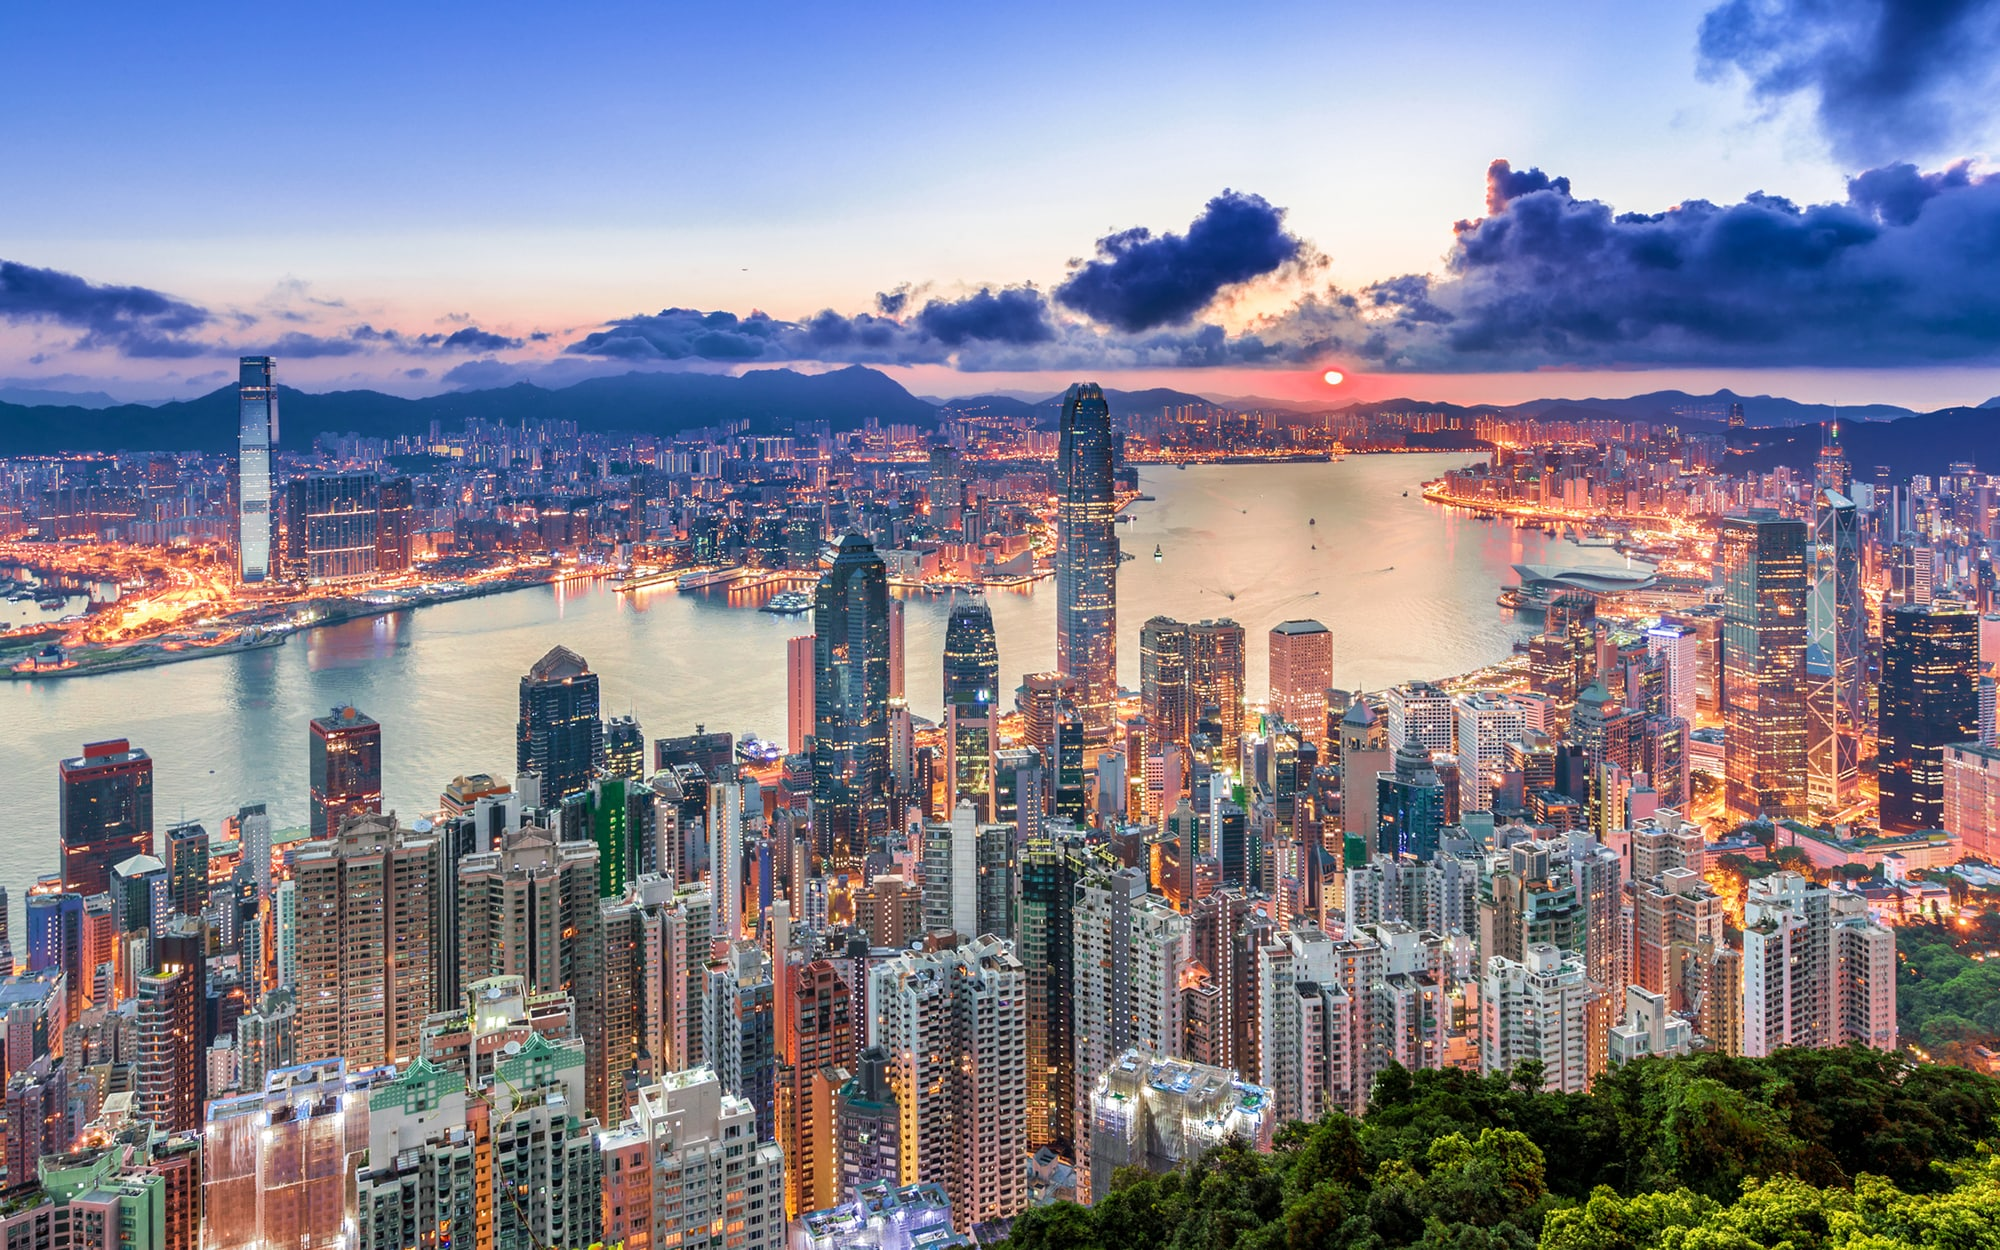
\includegraphics[width=1\textwidth,height=\textheight]{./figures/Hong-Kong.jpeg}

}

\caption{Hong Kong's skyline.
Source:https://www.telegraph.co.uk/content/dam/Travel/Destinations/Asia/Hong\%20Kong/hong-kong-victoria-peak-pano-guide.jpg}

\end{figure}

With interest in geospatial science, I have decided to pursue a Master's
degree related to it, hence, I am now studying the MSc Social and
Geographic Data Science at UCL. I am very new to programming, and it is
always a challenge for me to troubleshoot errors and problems in Rstudio
and python when performing different types of spatial analysis, and data
manipulation. I hope to improve and enhance my skills on geospatial
science in this degree. Besides, I want to learn more about remote
sensing, because I have not been taking many courses related to remote
sensing in the past. So, I hope I can learn about the principles and
important concepts in remote sensing, and utilize the knowledge in the
future. For each week, there will be summary and application example,
followed by a reflection, please enjoy.

\bookmarksetup{startatroot}

\hypertarget{week-1}{%
\chapter{Week 1}\label{week-1}}

Remote sensing in short is the detection and monitoring of the earth or
a certain area through measurements of the reflected and emitted
radiation at a distance. There are various types of remote sensing
instruments, and there are 2 types of them, including active sensor and
passive sensor.

\begin{itemize}
\item
  Active Sensors: Contain own energy source for illumination. They
  illuminate target objects and actively send pulses and measure the
  backscatters reflected to them. Synthetic Aperture Radar (SAR) and
  laser fluorosensor are examples of active sensors.
\item
  Passive Sensors: Do not have any illuminating source. They detect and
  reflect energy when it is naturally available, and only take place
  during the time when the sun is illuminating the Earth. Passive
  infrared sensor (PIR) and radiometers are examples of passive sensors.
\end{itemize}

The aforementioned term of ``energy'' is concisely referring to the
energy emitted from the sun, which comes as Electromagnetic radiation
(EMR) or Electromagnetic waves (EM waves) to the earth. They are waves
of magnetic and electric fields spreading across different wavelength
from very short gamma rays, x-ray to infrared waves, and micro waves
etc. EM waves travel through vacuum of space at constant speed of light.

\begin{figure}

{\centering 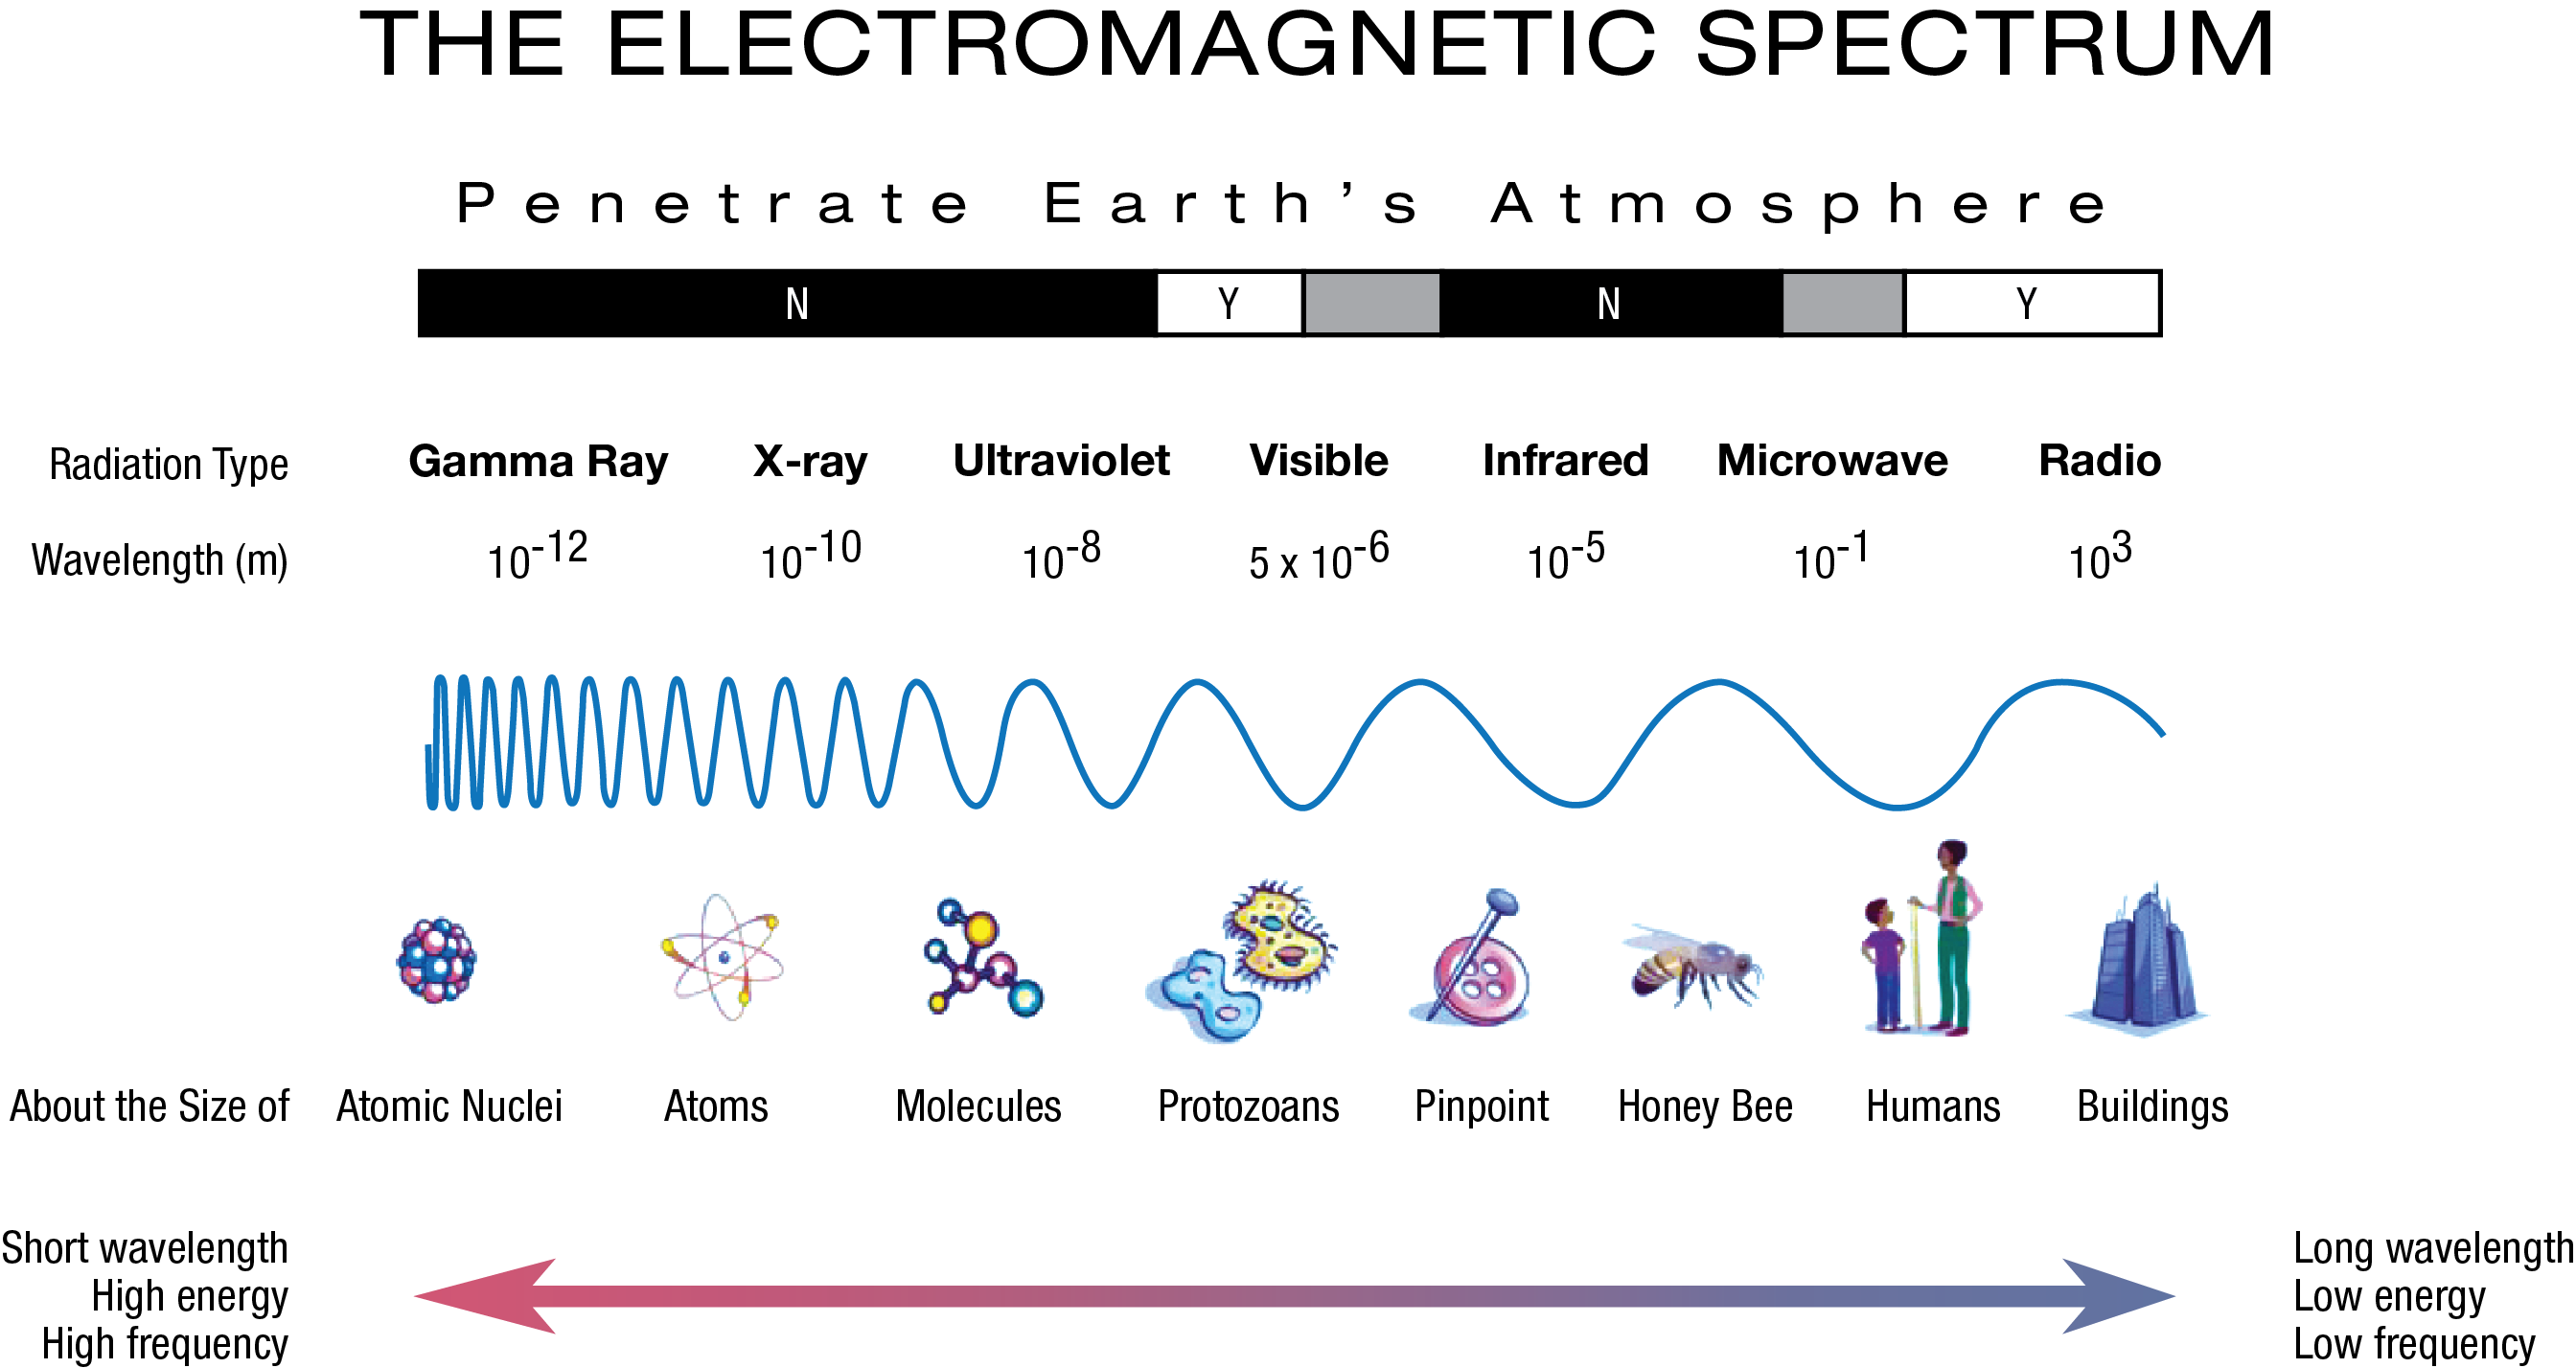
\includegraphics[width=0.7\textwidth,height=\textheight]{./figures/electromagnetic spectrum.png}

}

\caption{The Electromagnetic Spectrum.
Source:https://mynasadata.larc.nasa.gov/basic-page/electromagnetic-spectrum-diagram}

\end{figure}

Before EMR is received by sensors, several processes and changes are
required before hitting the sensors, including energy absorption by the
surface, transmission through surface and scattering by particles in the
atmosphere.

In practical 1, sentinel products were used. It is a product that has
been processed through multi-spectral imagery. The spectral imagery is
one of the four resolutions used in all remotely sensed data, it
contains layer of different bands. I have chosen the Zeeland province of
the Netherlands, it is located in the southwestern part consisting
islands and peninsulas which are interconnected by the dams and bridges
of the Delta Works.

\begin{figure}

{\centering 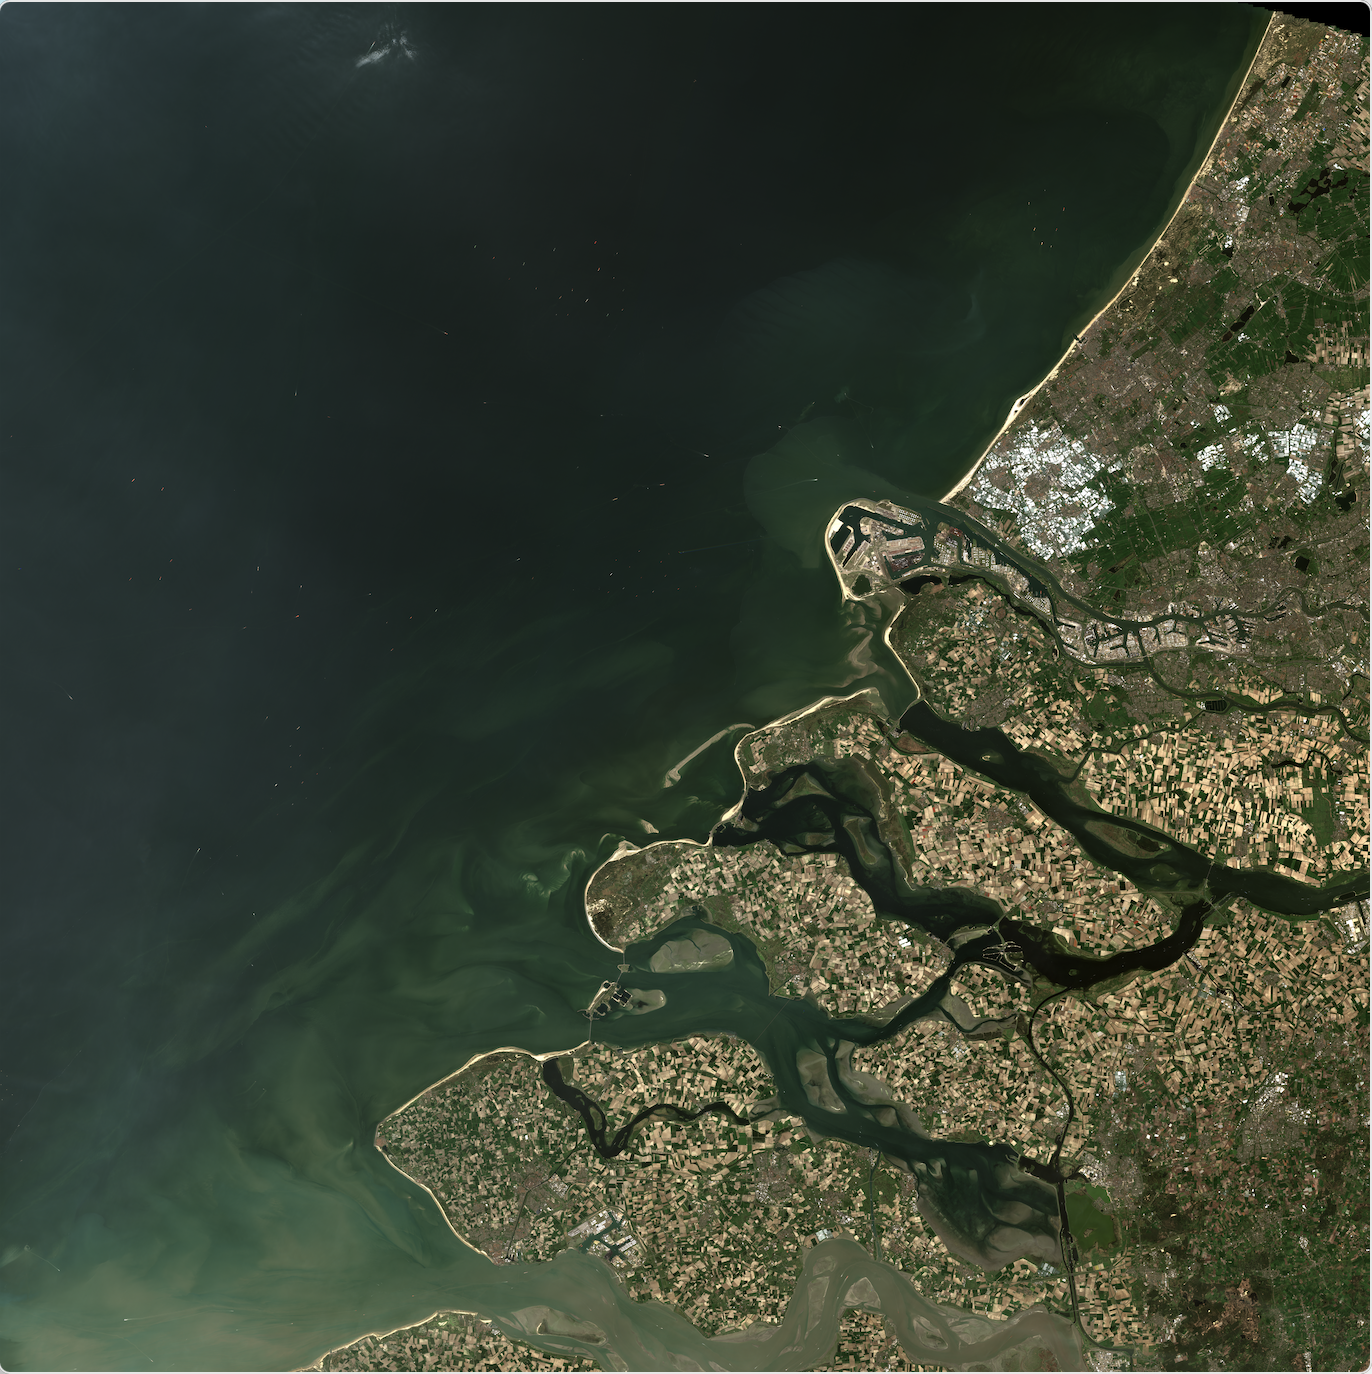
\includegraphics[width=1\textwidth,height=\textheight]{./figures/Screenshot 2023-02-08 at 4.13.36 PM.png}

}

\end{figure}

This figure shown above is a True Color Image (TCI) that contains B02,
B03 and B04 for blue, green and red bands. Yet, the image remain a
single raster layer that has a limited value from 0 - 255. In order to
enhance the resolution for the sentinel product that has higher much
higher brightness level, a raster band could be made manually with the
existing separate bands from the Sentinel-2 Level-2A product.

\begin{figure}

{\centering \includegraphics[width=1\textwidth,height=\textheight]{./figures/Screenshot 2023-02-07 at 5.14.55 PM.png}

}

\end{figure}

As shown in the figure, I have recreated the true color composite using
the RGB window, selecting band B04 , B03 and B02 for red, green and blue
respectively. The image colour is slightly different from the TCI
because I have used the `Colour Manipulation' function to change the
distribution of the three bands. The scatter plot on the left shows B04
against B08, which implies the vegetation cover of the area. As the
y-axis is the near-infrared reflectance, and x-axis is the red band,
high values of y and low values of x in the plot represents dense canopy
while low values of both x and y are most likely wet bare soil. From the
graph, the image contains little vegetation cover and more soil that is
wet and bare.

\hypertarget{application}{%
\section{Application}\label{application}}

While remote sensors detect, quantify and record the EM energy, the
captured satellite images are geo-referenced. One of the most common
applications is land cover remote sensing analysis. According to Aplin
(2004), different land cover features reflect EM radiation differently,
hence, the distinctive radiation provides the representations of land
cover variation. As passive sensors require external illumination
source, they are dependent to the sun as a source of light and are
limited by various conditions. Tempfli et al. (2009) stated that at
conditions like during nighttime, when solar radiation is absent and in
areas that are mostly covered under clouds, remote sensors are useless.
On the contrary, active sensors that have their own source of
illumination can operate at any time because they are can emit EM energy
and detect the energy returning from the target object or surface.

Sentinel-2A Level 2A products provide Bottom Of Atmosphere (BOA)
reflectance images derived from the associated Level-1C products that
provide Top-Of-Atmosphere (TOA) reflectance. The Sentinel 2 product has
13 bands of data in 10, 20 and 60 meters pixel size respectively and
carries the Multispectral Imager (MSI). B04, B03 and B02 represent Red,
Green and Blue respectively, the combination of these 3 bands creates a
natural colour imagery that resembles the same way our eyes visualize
the real world.

\begin{figure}

{\centering 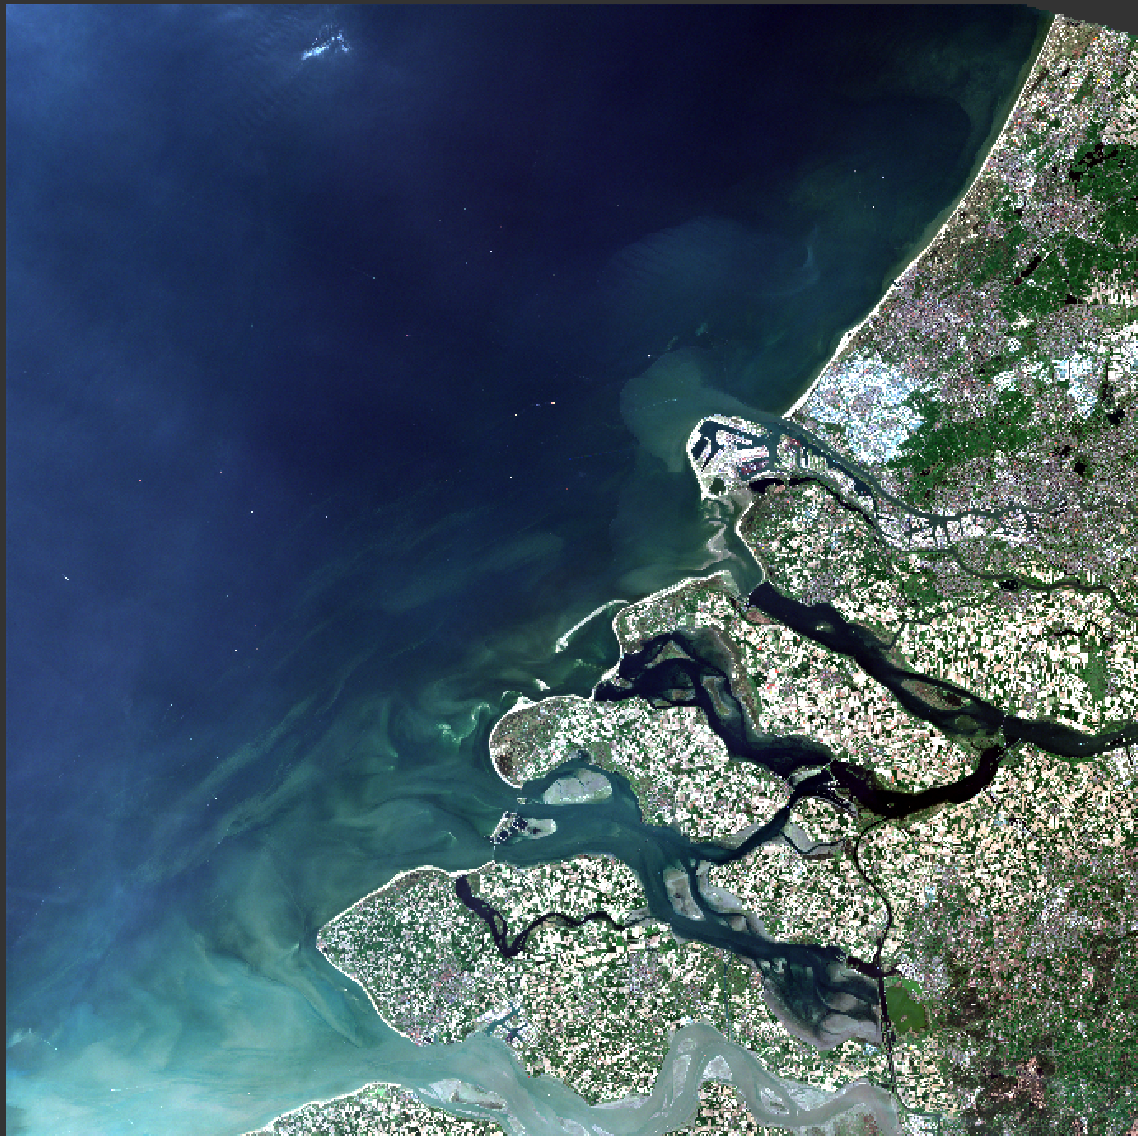
\includegraphics[width=1\textwidth,height=\textheight]{./figures/Screenshot 2023-02-08 at 9.10.51 PM.png}

}

\end{figure}

In this image, urban features tend to appear in white and grey, while
water is dark blue and vegetation is green. This image is very similar
to the TCI provided in the data downloaded

As vegetation strongly reflects near-infrared radiation and absorbs red
light, rather than generating aa vegetation index ((B8-B4)/(B8+B4)), a
scatter plot of B8 against B4 can also reflect vegetation of the image.
From the figure below, the ``Tasseled Cap'' shape is created. It reveals
that vegetation does not contribute big proportion in the image as the
zone of low red and high near infrared values are narrow. Instead, many
values concentrate at the low red and low infrared regions, showing that
water is present and has higher ratio in the image. Referring back to
the image, it is true that the image contains both land and sea. In
addition, the values of higher red band values indicate that vegetation
decreases as their presence can absorb red bands. Large part of the
image that are not ocean is developed and built area.

\begin{figure}

{\centering 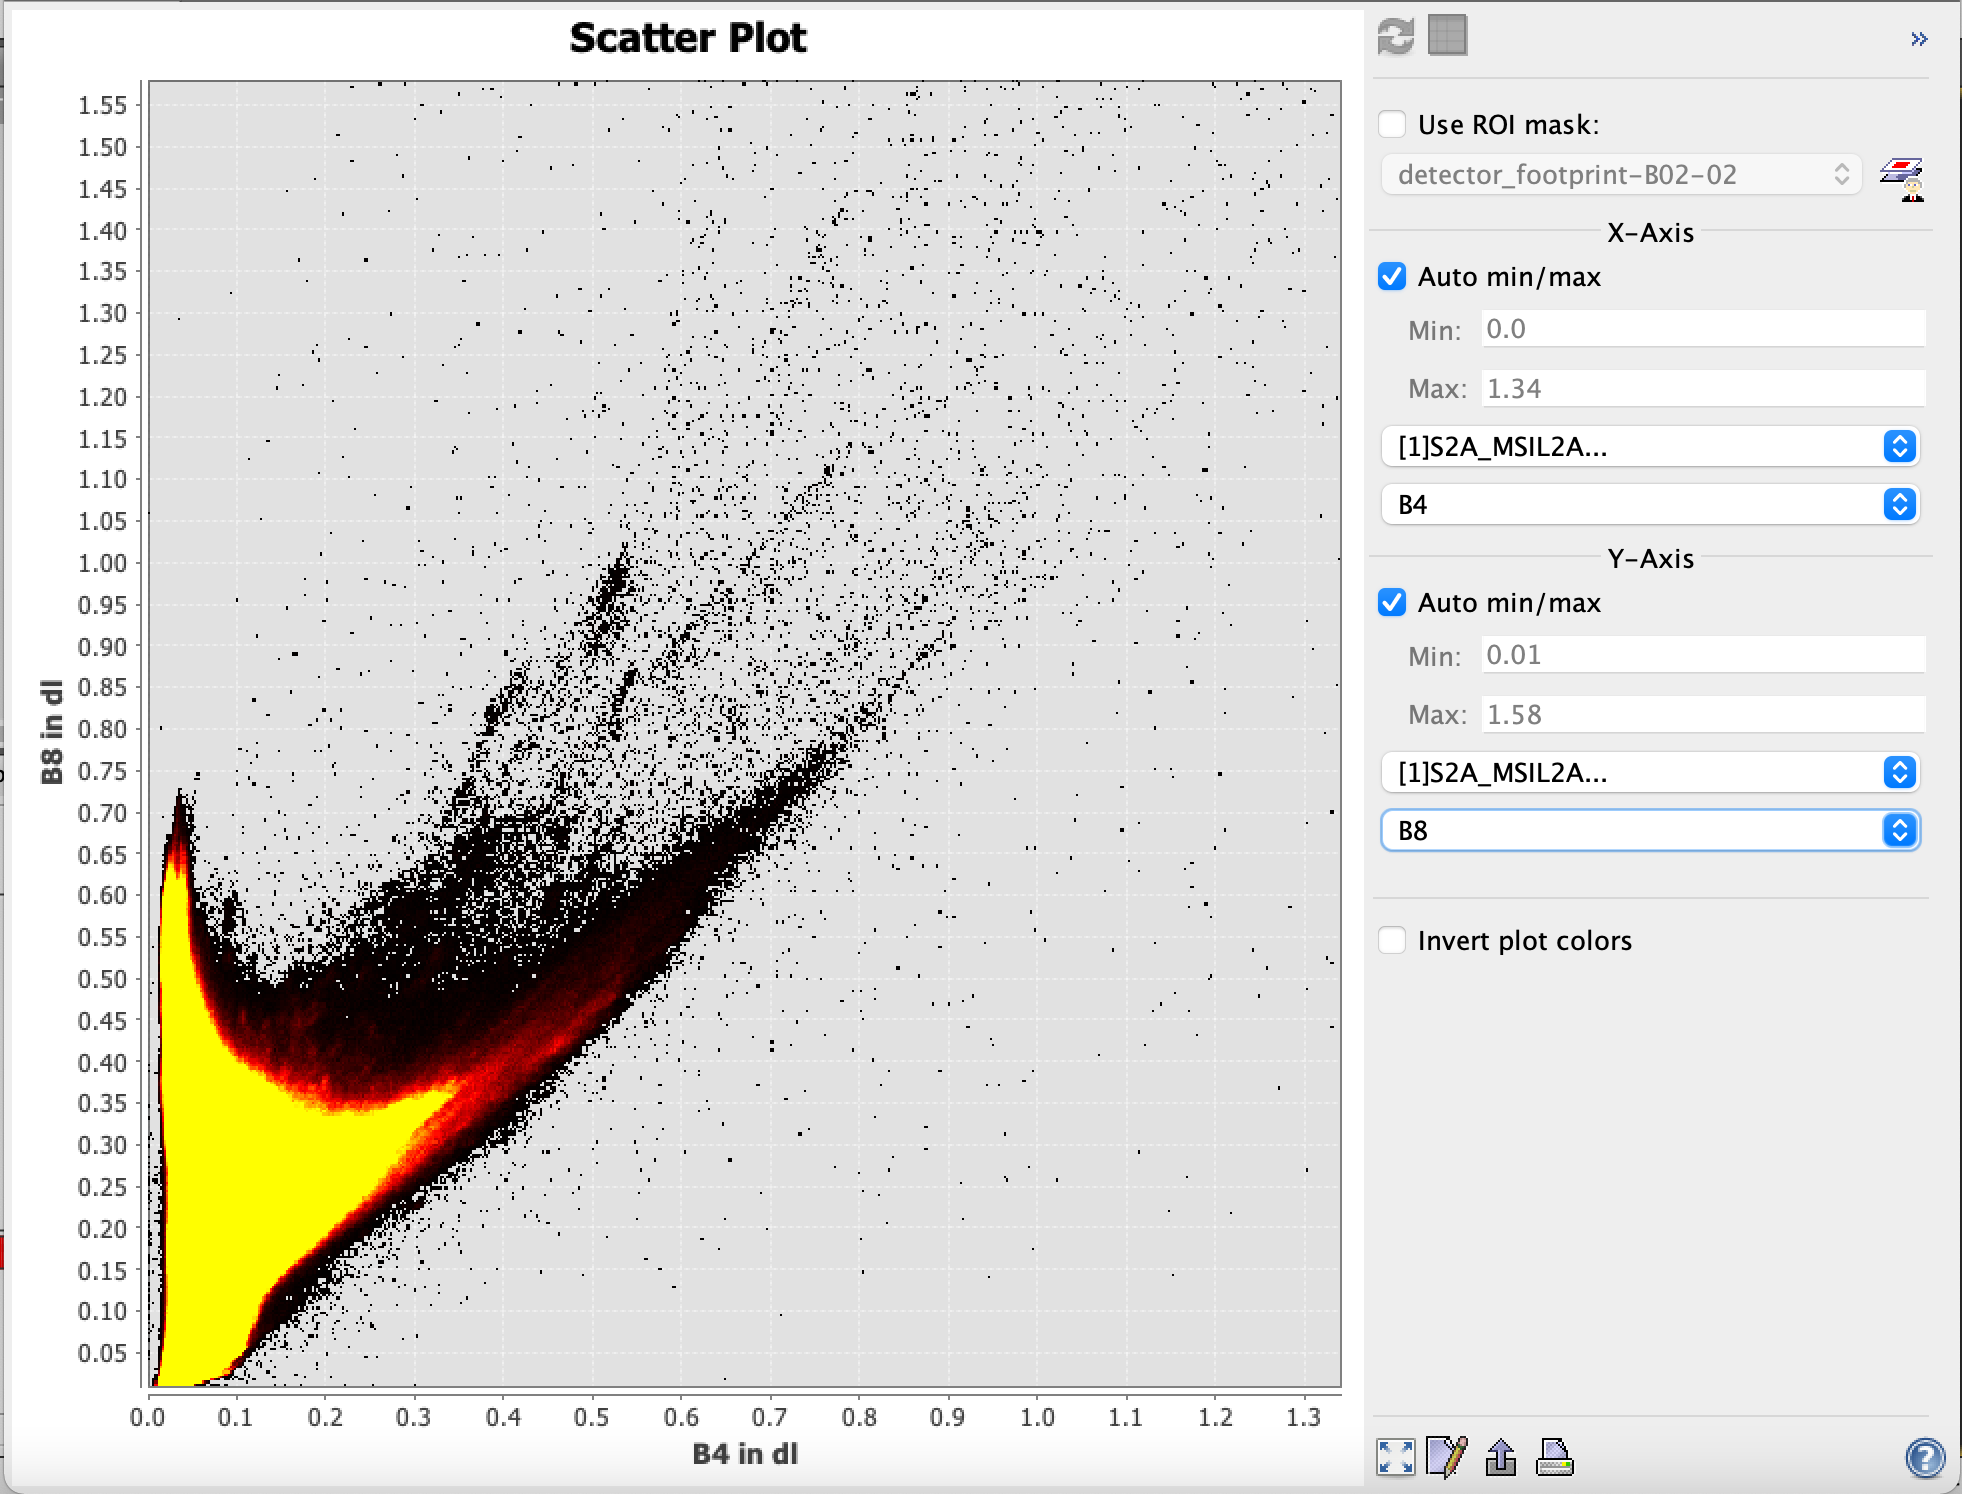
\includegraphics[width=1\textwidth,height=\textheight]{./figures/Screenshot 2023-02-08 at 9.15.03 PM.png}

}

\end{figure}

\hypertarget{reflection}{%
\section{Reflection}\label{reflection}}

I personally think that remote sensing is way more useful and
complicated than it sounds. As I have always focused on learning how to
manipulate and wrangle vector data in GIS, I seldom use satellite images
as I thought it would only be an image that shows the land features
succinctly. However, this practical has definitely made me realized that
satellite images could do more than that. I am especially interested
with the multispectral bands in the sentinel 2 product. The different
combinations of bands could create and reveal different information from
an image. Other than the natural colour of \textbf{B4, B3 and B2}, there
are many different combination. With knowledge on what land features
absorb and reflect, the combinations could create images that allow
classifcation of land features in a more detailed manner. For example,
colour infrared image of \textbf{B8, B4 and B3} can reveal healthy and
unhealthy vegetation as near-infrared band is good at reflecting
chlorpophyll. A Bathymetric image of \textbf{B4, B3 and B1} is
favourable for coastal studies as the coastal aerosol band can estimate
suspended sediment in water more accurately. Also, a moisture index
image composed of \textbf{(B8A-B11)/(B8A+B11)} can reveal moisture
content and perhaps water stress in plants. There are still a lot of
combinations of bands, I think it is especially useful for people to
gain a brief understanding to a specific area before actually go on a
site visit.

\bookmarksetup{startatroot}

\hypertarget{week-2}{%
\chapter{Week 2}\label{week-2}}

In week 2, we have learnt about concepts in Xanringan and Quarto and the
weekly task is to create both documents

\bookmarksetup{startatroot}

\hypertarget{week-3}{%
\chapter{Week 3}\label{week-3}}

Raw remote sensing images are known to have notable distortions and
flaws, which is mainly caused by the curved Earth, incompletely
transparent atmosphere, varying solar radiation throughout the day and
limitations of instruments. Therefore, most of the raw data captured by
remote sensors are preprocessed to remove most of the flaws, it is
called \textbf{Image Correction.}

Below shows a summary of 4 different correction methods, including
\textbf{Geometric correction, Atmospheric correction, Orthorectification
correction} and \textbf{Radiometric correction.}

\begin{figure}

{\centering 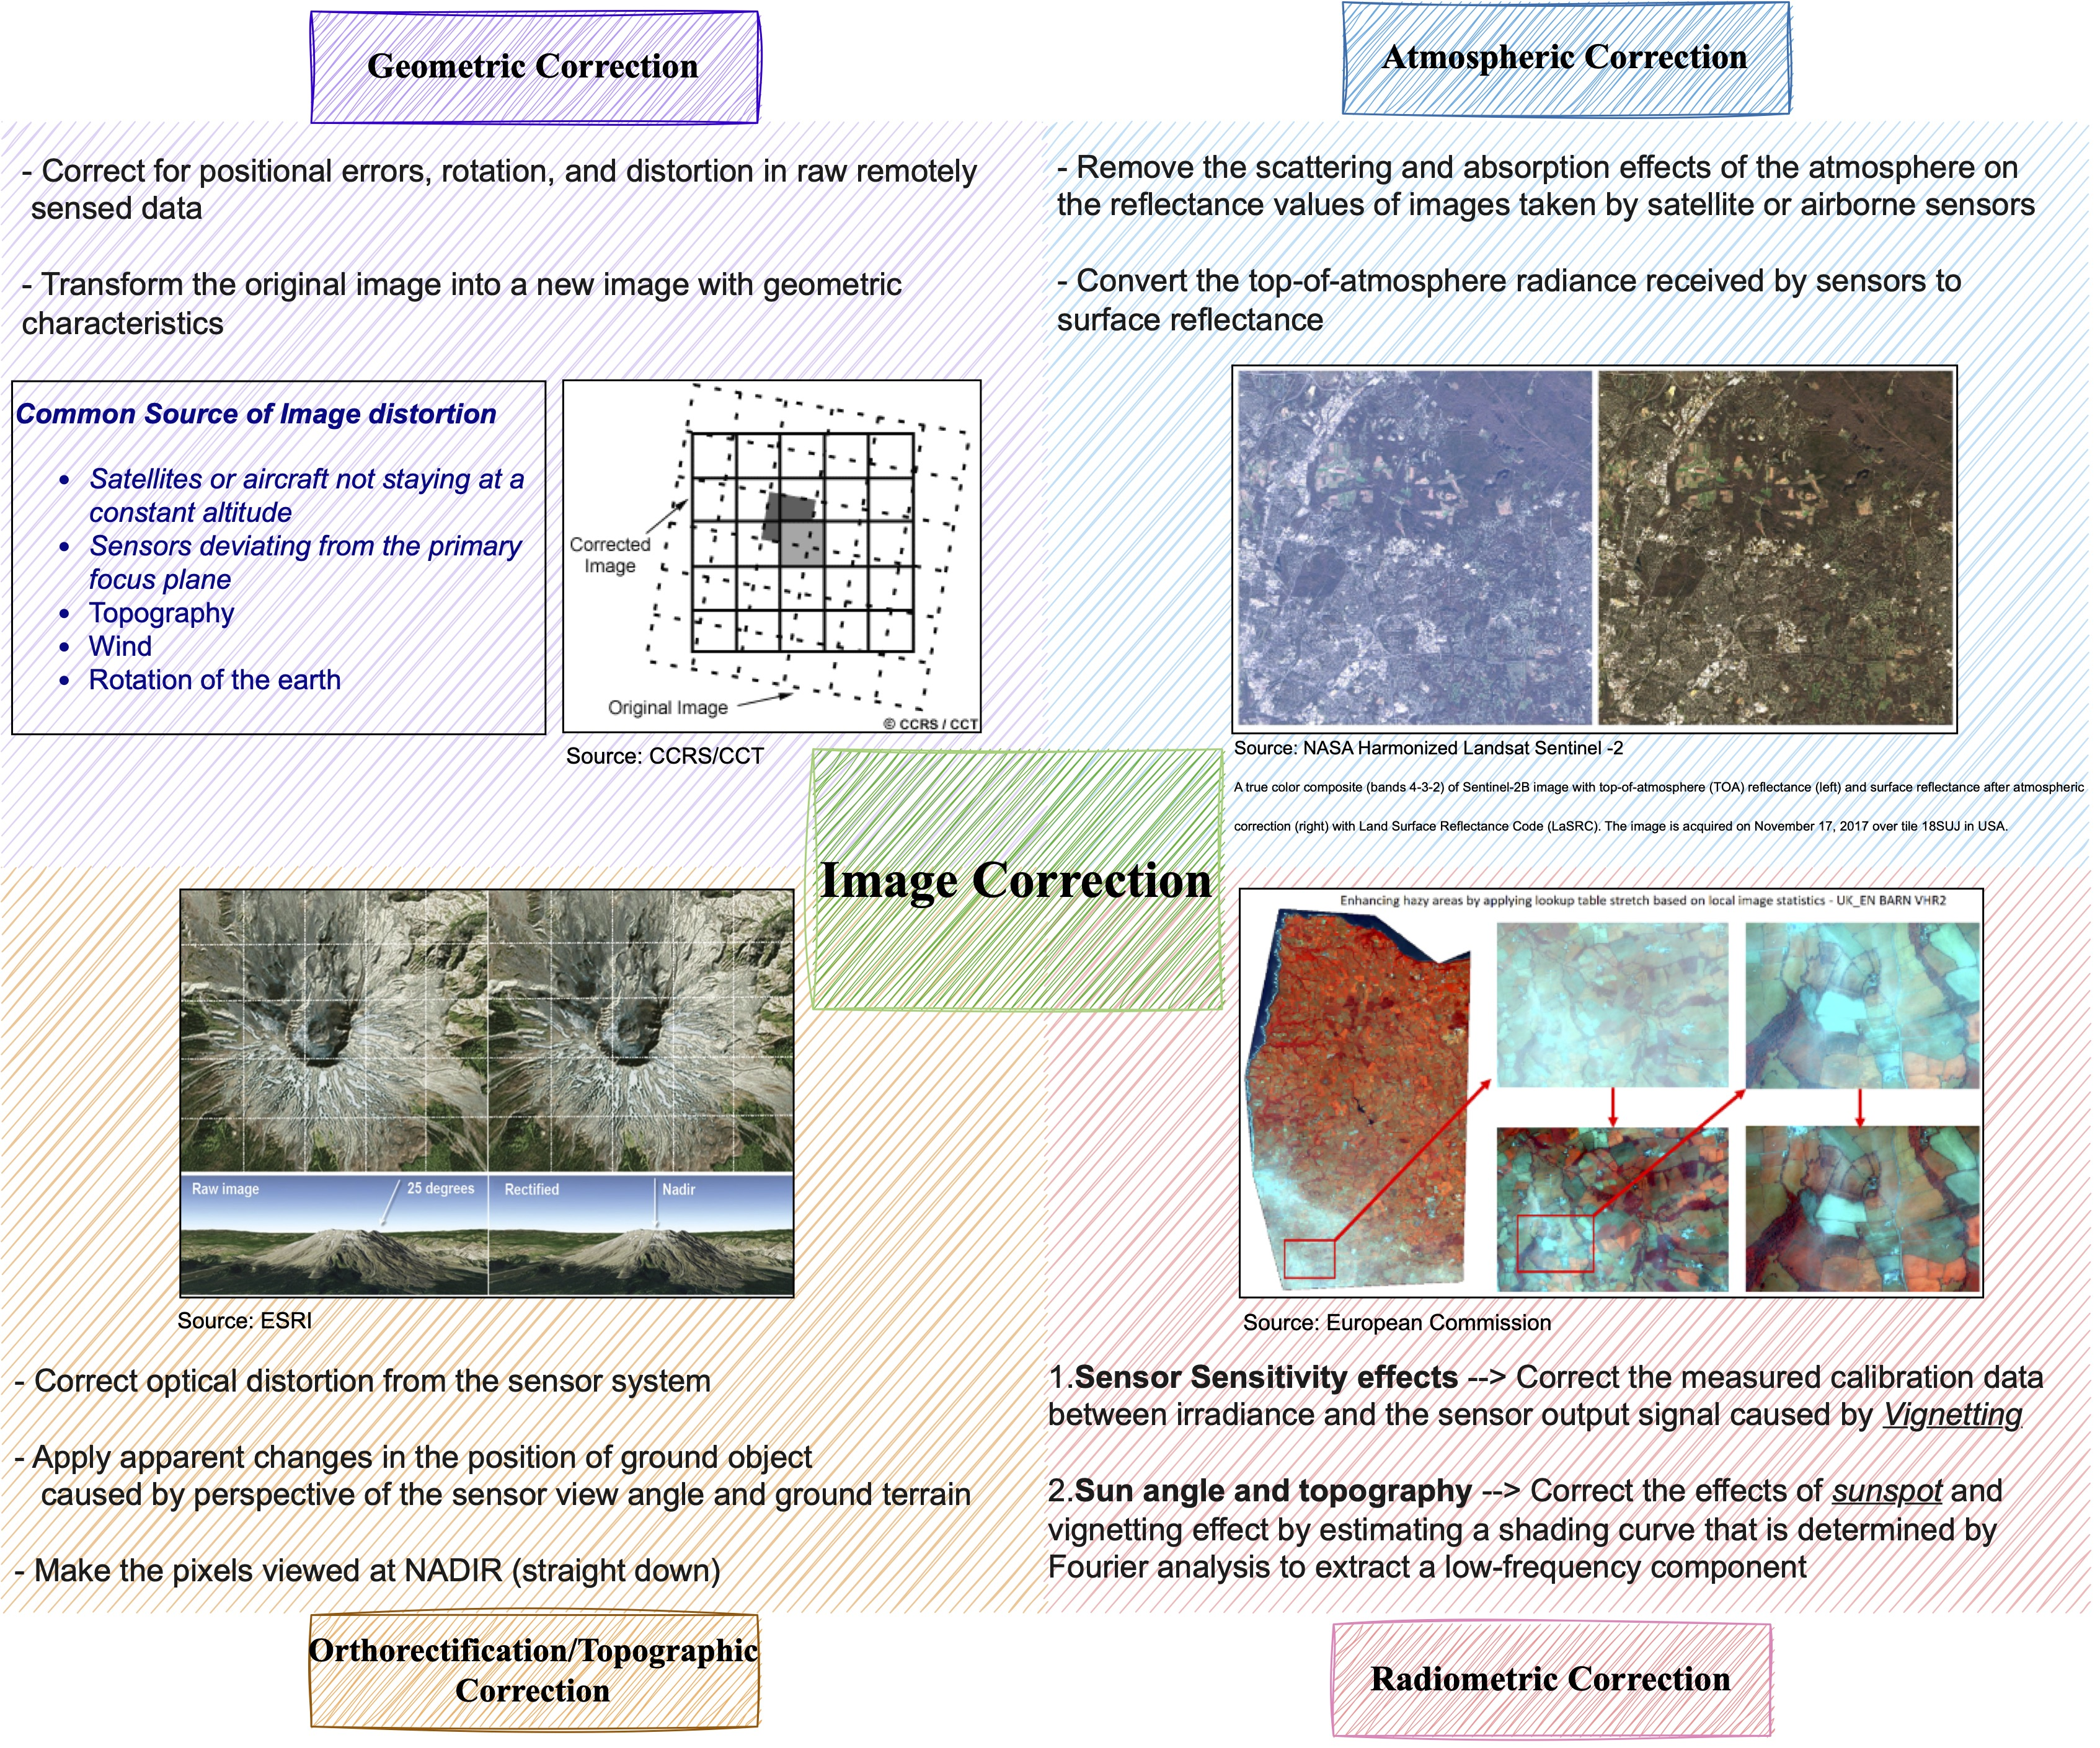
\includegraphics[width=1\textwidth,height=\textheight]{./figures/correction summary.jpg}

}

\end{figure}

\hypertarget{application-1}{%
\section{Application}\label{application-1}}

\hypertarget{reflection-1}{%
\section{Reflection}\label{reflection-1}}

\bookmarksetup{startatroot}

\hypertarget{week-4}{%
\chapter{Week 4}\label{week-4}}

Geometric correction is used to correct positional errors and to
transform original image to a new image

\hypertarget{application-2}{%
\section{Application}\label{application-2}}

\hypertarget{reflection-2}{%
\section{Reflection}\label{reflection-2}}

\bookmarksetup{startatroot}

\hypertarget{week-5}{%
\chapter{Week 5}\label{week-5}}

Geometric correction is used to correct positional errors and to
transform original image to a new image

\hypertarget{application-3}{%
\section{Application}\label{application-3}}

\hypertarget{reflection-3}{%
\section{Reflection}\label{reflection-3}}

\bookmarksetup{startatroot}

\hypertarget{week-6}{%
\chapter{Week 6}\label{week-6}}

Geometric correction is used to correct positional errors and to
transform original image to a new image

\hypertarget{application-4}{%
\section{Application}\label{application-4}}

\hypertarget{reflection-4}{%
\section{Reflection}\label{reflection-4}}

\bookmarksetup{startatroot}

\hypertarget{week-7}{%
\chapter{Week 7}\label{week-7}}

Geometric correction is used to correct positional errors and to
transform original image to a new image

\hypertarget{application-5}{%
\section{Application}\label{application-5}}

\hypertarget{reflection-5}{%
\section{Reflection}\label{reflection-5}}

\bookmarksetup{startatroot}

\hypertarget{week-8}{%
\chapter{Week 8}\label{week-8}}

Geometric correction is used to correct positional errors and to
transform original image to a new image

\hypertarget{application-6}{%
\section{Application}\label{application-6}}

\hypertarget{reflection-6}{%
\section{Reflection}\label{reflection-6}}

\bookmarksetup{startatroot}

\hypertarget{summary}{%
\chapter{Summary}\label{summary}}

In summary, this book has no content whatsoever.

\begin{Shaded}
\begin{Highlighting}[]
\DecValTok{1} \SpecialCharTok{+} \DecValTok{1}
\end{Highlighting}
\end{Shaded}

\begin{verbatim}
[1] 2
\end{verbatim}

\bookmarksetup{startatroot}

\hypertarget{references}{%
\chapter*{References}\label{references}}
\addcontentsline{toc}{chapter}{References}

\markboth{References}{References}

\leavevmode\vadjust pre{\hypertarget{refs}{}}%
\begin{CSLReferences}{1}{0}
Aplin (2004)

Tempfli et al. (2009)

\leavevmode\vadjust pre{\hypertarget{ref-aplin2004}{}}%
Aplin, Paul. 2004. {``Remote Sensing: Land Cover.''} \emph{Progress in
Physical Geography: Earth and Environment} 28 (2): 283--93.
\url{https://doi.org/10.1191/0309133304pp413pr}.

\leavevmode\vadjust pre{\hypertarget{ref-tempfli2009}{}}%
Tempfli, Klaus, G. C. Huurneman, Wim Bakker, L. L. F. Janssen, W. F.
Feringa, Ambro Gieske, K. A. Grabmaier, et al. 2009. {``Principles of
Remote Sensing : An Introductory Textbook.''} In, 56--85.

\end{CSLReferences}



\end{document}
